\documentclass[11pt]{article}
\usepackage[utf8]{inputenc}
\usepackage[T1]{fontenc}
\usepackage{geometry, tikz, xcolor, enumitem, ragged2e}
\geometry{a4paper, margin=1.5cm}

\begin{document}

\begin{center}
\Large \textbf{\textcolor{blue!60!black}{Atividade: Matemática – Progressão Aritmética (PA)}}\\[0.3cm]
\large Professor: Jefferson
\end{center}

\vspace{0.3cm}
\large Nome: \underline{\hspace{8cm}} \quad Turma: \underline{\hspace{3cm}}

\vspace{0.5cm}

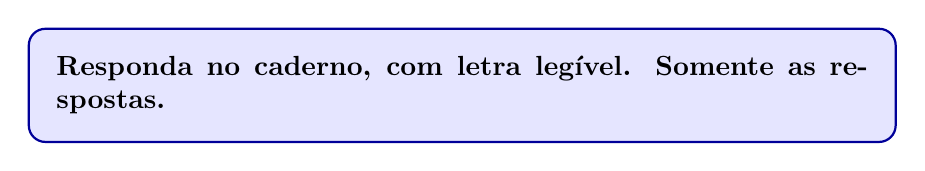
\begin{tikzpicture}
\node[rectangle, fill=blue!10, rounded corners=6pt, inner sep=10pt, draw=blue!60!black, thick]{
\begin{minipage}{0.85\linewidth}
\textbf{Responda no caderno, com letra legível. Somente as respostas.}
\end{minipage}
};
\end{tikzpicture}

\vspace{0.6cm}

\begin{enumerate}

\item Explique, com suas palavras, o que caracteriza uma sequência numérica como Progressão Aritmética.

\item O que chamamos de \textbf{razão} de uma PA? Descreva como ela pode ser encontrada.

\item Qual a diferença entre uma PA crescente, decrescente e constante? Cite um exemplo de cada.

\item Na fórmula do termo geral $a_n = a_1 + (n-1)r$, explique o significado de cada elemento ($a_n$, $a_1$, $n$, $r$).

\item Em uma PA, se conhecemos dois termos não consecutivos, como podemos descobrir a razão? Descreva o procedimento.

\item Por que a soma dos termos de uma PA pode ser calculada usando a média entre o primeiro e o último termo? Explique o raciocínio.

\item Em que situações do cotidiano uma Progressão Aritmética pode aparecer? Cite pelo menos dois exemplos.

\item Explique por que toda PA possui comportamento de crescimento ou decrescimento linear, e não exponencial.

\item Calcule o 10º termo da PA: $3, 7, 11, 15, \dots$

\item Uma PA tem primeiro termo $a_1 = 12$ e razão $r = -3$. Determine o 8º termo.

\item Encontre a soma dos 15 primeiros termos da PA: $5, 8, 11, \dots$

\item Se o 5º termo de uma PA é 20 e o 12º termo é 41, determine o primeiro termo e a razão.


\end{enumerate}

\vspace{1cm}
\textbf{\Large Gabarito (Respostas-modelo)}

\begin{enumerate}

\item Uma sequência é uma PA quando a diferença entre um termo e o termo anterior é sempre constante.

\item A razão é o valor que se soma (ou subtrai) para passar de um termo ao próximo. Calcula-se fazendo $r = a_{n} - a_{n-1}$.

\item PA crescente: $r > 0$ (ex.: $2, 5, 8, 11,\dots$).  
PA decrescente: $r < 0$ (ex.: $20, 15, 10, 5,\dots$).  
PA constante: $r = 0$ (ex.: $7, 7, 7, 7,\dots$).

\item $a_n$ é o termo desejado; $a_1$ é o primeiro termo; $n$ é a posição do termo; $r$ é a razão da PA.

\item Podemos usar $a_n = a_1 + (n-1)r$ para montar duas equações e resolver o sistema para encontrar $r$.

\item Porque a soma de uma PA pode ser reorganizada em pares onde cada par soma o mesmo valor. Por isso, $S_n = \frac{n(a_1 + a_n)}{2}$.

\item Exemplos: depósitos mensais sempre com o mesmo acréscimo; preços que aumentam um mesmo valor ao longo dos meses; tabelas salariais com reajuste fixo.

\item Porque em uma PA sempre adicionamos um valor constante a cada passo, o que gera variação linear, não multiplicativa (que seria exponencial).

\item $a_{10} = a_1 + (10-1)r = 3 + 9\cdot 4 = 39$

\item $a_8 = 12 + (8-1)(-3) = 12 - 21 = -9$

\item $S_{15} = \frac{15(5 + 5 + (15-1)\cdot 3)}{2} = \frac{15(5 + 47)}{2} = \frac{15 \cdot 52}{2} = 390$

\item $a_5 = a_1 + 4r = 20 \Rightarrow a_1 + 4r = 20$  
    $a_{12} = a_1 + 11r = 41 \Rightarrow a_1 + 11r = 41$  
    Subtraindo: $7r = 21 \Rightarrow r = 3$  
    Então $a_1 + 4\cdot 3 = 20 \Rightarrow a_1 = 8$


\end{enumerate}

\end{document}

